\documentclass{beamer}
\usetheme{Madrid}
\usecolortheme{dolphin}
\usepackage{amsmath}
\usepackage{amssymb}
\usepackage{graphicx}
\usepackage{tikz}
\usepackage{algorithm}
\usepackage{algorithmic}
\usepackage{booktabs}
\usepackage{multirow}
\usepackage{xcolor}

\title{Reinforcement learning for Integrated Fixed-income with Link-based Embeddings}
\subtitle{Integrating Regime Detection, Graph Neural Networks, and Modern RL Algorithms}
\author{Corentin Servouze, Rany Stephan}
\date{\today}

\begin{document}

\begin{frame}
\titlepage
\end{frame}

\begin{frame}{Outline}
\tableofcontents
\end{frame}

%----------------------------------------------------------
\section{Introduction}
%----------------------------------------------------------

\begin{frame}{The Problem of Fixed Income Portfolio Management}
\begin{itemize}
    \item \textbf{Fixed income markets} represent over \$100 trillion globally
    \item Managing bond portfolios involves complex challenges:
    \begin{itemize}
        \item Interest rate risk and credit risk management
        \item Multi-dimensional features (duration, convexity, credit quality)
        \item Regime-dependent dynamics (recession, expansion, crisis)
        \item Limited liquidity compared to equities
    \end{itemize}
    \item Traditional approaches:
    \begin{itemize}
        \item Static allocation strategies (ladders, barbells)
        \item Duration targeting
        \item Factor-based or index-tracking methods
    \end{itemize}
\end{itemize}
\end{frame}



\begin{frame}{Project Innovation}
\begin{itemize}
    \item Comprehensive RL framework for fixed income portfolios that:
    \begin{itemize}
        \item Integrates regime detection for regime-aware strategies
        \item Incorporates credit risk through graph neural networks
        \item Uses RL algorithms (TD3, DDPG)
        \item Models realistic bond market dynamics
    \end{itemize}
    \item Creates a complete simulation-to-deployment pipeline
    \item Addresses multi-faceted bond portfolio optimization with focus on risk-adjusted returns
\end{itemize}
\end{frame}

%----------------------------------------------------------
\section{Project Overview}
%----------------------------------------------------------

\begin{frame}{Project Architecture}
\centering
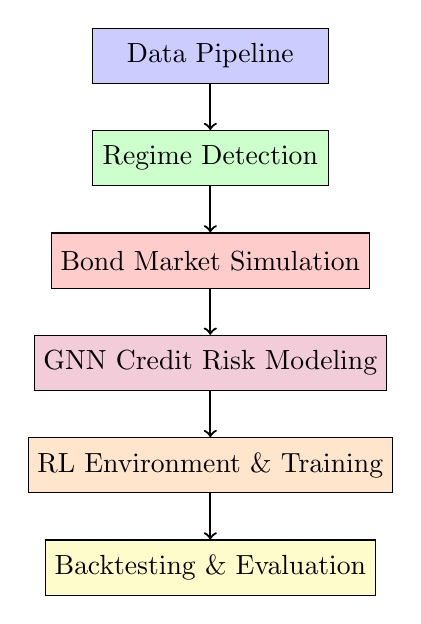
\begin{tikzpicture}[node distance=1.3cm]
\node (data) [draw, rectangle, minimum width=3cm, minimum height=0.7cm, fill=blue!20] {Data Pipeline};
\node (regime) [draw, rectangle, minimum width=3cm, minimum height=0.7cm, fill=green!20, below of=data] {Regime Detection};
\node (market) [draw, rectangle, minimum width=3cm, minimum height=0.7cm, fill=red!20, below of=regime] {Bond Market Simulation};
\node (gnn) [draw, rectangle, minimum width=3cm, minimum height=0.7cm, fill=purple!20, below of=market] {GNN Credit Risk Modeling};
\node (rl) [draw, rectangle, minimum width=3cm, minimum height=0.7cm, fill=orange!20, below of=gnn] {RL Environment \& Training};
\node (backtest) [draw, rectangle, minimum width=3cm, minimum height=0.7cm, fill=yellow!20, below of=rl] {Backtesting \& Evaluation};

\draw[->, thick] (data) -- (regime);
\draw[->, thick] (regime) -- (market);
\draw[->, thick] (market) -- (gnn);
\draw[->, thick] (gnn) -- (rl);
\draw[->, thick] (rl) -- (backtest);
\end{tikzpicture}

\end{frame}

\begin{frame}{Sample Data Visualization}
    \centering
    \includegraphics[width=\textwidth]{../output/ppt0.png}
\end{frame}


\begin{frame}{Prior Work in Fixed Income RL}
\begin{itemize}
    \item Limited research compared to equity RL applications
    \item Notable prior work:
    \begin{itemize}
        \item Halperin \& Feldshteyn (2018): Q-learning for fixed income trading
        \item Kolm \& Ritter (2019): Deep hedging with neural networks
        \item Makinen et al. (2019): RL for corporate bond trading
    \end{itemize}
    \item Limitations of existing approaches:
    \begin{itemize}
        \item Often simplified market dynamics
        \item Limited consideration of regime changes
        \item Lack of network effects in credit risk
        \item Focus on single bonds rather than portfolios
    \end{itemize}
\end{itemize}
\end{frame}

%----------------------------------------------------------
\section{Bond Market Models}
%----------------------------------------------------------

\begin{frame}{Interest Rate Models}
\begin{itemize}
    \item \textbf{Vasicek Model}:
    \begin{equation}
    dr_t = \kappa(\theta - r_t)dt + \sigma dW_t
    \end{equation}
    where:
    \begin{itemize}
        \item $r_t$ is the short rate at time $t$
        \item $\kappa$ is the mean reversion speed
        \item $\theta$ is the long-term mean level
        \item $\sigma$ is the volatility
        \item $dW_t$ is a Wiener process increment
    \end{itemize}
    \item Mean-reverting process capturing central tendency of rates
    \item Allows for negative rates (theoretical limitation)
\end{itemize}
\end{frame}

\begin{frame}{Interest Rate Models (Continued)}
\begin{itemize}
    \item \textbf{Cox-Ingersoll-Ross (CIR) Model}:
    \begin{equation}
    dr_t = \kappa(\theta - r_t)dt + \sigma\sqrt{r_t}dW_t
    \end{equation}
    \begin{itemize}
        \item Square root diffusion term ensures non-negative rates
        \item Higher volatility when rates are higher
        \item Same mean-reversion structure as Vasicek
    \end{itemize}
    
    \item \textbf{Hull-White Model}:
    \begin{equation}
    dr_t = [\theta(t) - \kappa r_t]dt + \sigma dW_t
    \end{equation}
    \begin{itemize}
        \item Time-dependent $\theta(t)$ function
        \item Calibrated to match initial yield curve
        \item Extension of Vasicek with greater flexibility
    \end{itemize}
\end{itemize}
\end{frame}

\begin{frame}{Credit Spread Models}
\begin{itemize}
    \item \textbf{Merton Model}:
    \begin{itemize}
        \item Firm's asset value $V$ follows geometric Brownian motion:
        \begin{equation}
        dV_t = rV_tdt + \sigma_V V_t dW_t
        \end{equation}
        \item Default occurs if $V_T < D$ at debt maturity $T$
        \item Credit spread:
        \begin{equation}
        s(t,T) = -\frac{1}{T-t}\ln(1 - N(-d_2))
        \end{equation}
        where $d_2 = \frac{\ln(V_t/D) + (r-\frac{1}{2}\sigma_V^2)(T-t)}{\sigma_V\sqrt{T-t}}$
    \end{itemize}
    
    \item Model parameters:
    \begin{itemize}
        \item Asset value $V_t$
        \item Face value of debt $D$
        \item Asset volatility $\sigma_V$
        \item Risk-free rate $r$
    \end{itemize}
\end{itemize}
\end{frame}

\begin{frame}{Bond Pricing}
\begin{itemize}
    \item \textbf{Zero-coupon bond price}:
    \begin{equation}
    P(t,T) = \frac{F}{(1+y_{t,T})^{T-t}}
    \end{equation}
    where $F$ is face value, $y_{t,T}$ is yield
    
    \item \textbf{Coupon bond price}:
    \begin{equation}
    P(t,T) = \sum_{i=1}^n \frac{c \cdot F}{(1+y_{t,T}/m)^{m(t_i-t)}} + \frac{F}{(1+y_{t,T}/m)^{m(T-t)}}
    \end{equation}
    where $c$ is coupon rate, $m$ is payments per year
    
    \item \textbf{Credit-risky bond}:
    \begin{equation}
    P(t,T) = \sum_{i=1}^n \frac{c \cdot F}{(1+r_{t,t_i}+s_{t,t_i})^{t_i-t}} + \frac{F}{(1+r_{t,T}+s_{t,T})^{T-t}}
    \end{equation}
    where $r_{t,T}$ is risk-free rate, $s_{t,T}$ is credit spread
\end{itemize}
\end{frame}

\begin{frame}{Bond Risk Metrics}
\begin{itemize}
    \item \textbf{Macaulay Duration}:
    \begin{equation}
    D = \frac{\sum_{t=1}^{T} t \cdot CF_t \cdot (1+y)^{-t}}{\sum_{t=1}^{T} CF_t \cdot (1+y)^{-t}}
    \end{equation}
    
    \item \textbf{Modified Duration}:
    \begin{equation}
    D_{mod} = \frac{D}{1+y}
    \end{equation}
    
    \item \textbf{Convexity}:
    \begin{equation}
    C = \frac{\sum_{t=1}^{T} t(t+1) \cdot CF_t \cdot (1+y)^{-t}}{P \cdot (1+y)^2}
    \end{equation}
    
    \item \textbf{Price sensitivity to yield changes}:
    \begin{equation}
    \frac{\Delta P}{P} \approx -D_{mod} \cdot \Delta y + \frac{1}{2} \cdot C \cdot (\Delta y)^2
    \end{equation}
\end{itemize}
Metrics capture different aspects of interest rate risk
\end{frame}



%----------------------------------------------------------
\section{Regime Detection}
%----------------------------------------------------------

\begin{frame}{Economic Regimes in Fixed Income}
\begin{itemize}
    \item Different market regimes significantly impact fixed income:
    \begin{itemize}
        \item \textbf{Normal regime}: Steady growth, stable rates
        \item \textbf{Expansion regime}: Rising rates, flattening yield curve
        \item \textbf{Stress regime}: Flight to quality, widening credit spreads
        \item \textbf{Crisis regime}: Rate cuts, extreme volatility, liquidity issues
    \end{itemize}
    \item \textbf{Importance for bond investors}:
    \begin{itemize}
        \item Risk factors behave differently across regimes
        \item Optimal allocations vary by regime
        \item Regime shifts create both risks and opportunities
        \item Traditional mean-variance assumptions break down during transitions
    \end{itemize}
\end{itemize}
\end{frame}

\begin{frame}{Hidden Markov Models for Regime Detection}
\begin{itemize}
    \item \textbf{Hidden Markov Model (HMM)} framework:
    \begin{itemize}
        \item Observable features $\mathbf{X}_t$ (yields, spreads, etc.)
        \item Hidden states (regimes) $z_t \in \{1,2,...,K\}$
        \item Emission distributions $p(\mathbf{X}_t|z_t)$
        \item Transition matrix $A$ where $A_{ij} = p(z_t=j|z_{t-1}=i)$
    \end{itemize}
    \item \textbf{Model specification}:
    \begin{equation}
    p(\mathbf{X}_t|z_t=k) = \mathcal{N}(\boldsymbol{\mu}_k, \boldsymbol{\Sigma}_k)
    \end{equation}
    \item \textbf{Parameter estimation} via Expectation-Maximization:
    \begin{itemize}
        \item E-step: Calculate posterior $p(z_t|X_{1:T})$ using forward-backward algorithm
        \item M-step: Update $\boldsymbol{\mu}_k$, $\boldsymbol{\Sigma}_k$, and $A$
    \end{itemize}
\end{itemize}
\end{frame}


%add image of hmm in latex 
\begin{frame}{Regime Detection Visualization}
    \centering
    \includegraphics[width=\textwidth]{../output/ppt1.png}
\end{frame}

\begin{frame}{Regime Characterization and Transitions}
\begin{itemize}
    \item \textbf{Statistical regime characteristics}:
    \begin{itemize}
        \item Expected returns, volatilities, correlations
        \item Yield curve shapes (normal, flat, inverted)
        \item Average spread levels by rating
        \item Typical duration of each regime (persistence)
    \end{itemize}
    \item \textbf{Transition matrix visualization}:
    
    \begin{center}
    \scriptsize
    \begin{tabular}{l|cccc}
    \toprule
    & Normal & Expansion & Stress & Crisis \\
    \midrule
    Normal & 0.983 & 0.010 & 0.005 & 0.002 \\
    Expansion & 0.015 & 0.975 & 0.008 & 0.002 \\
    Stress & 0.008 & 0.005 & 0.967 & 0.020 \\
    Crisis & 0.010 & 0.000 & 0.025 & 0.965 \\
    \bottomrule
    \end{tabular}
    \end{center}
    
    \item \textbf{Regime forecasting}:
    \begin{itemize}
        \item Short-term prediction via Markov property
        \item Confidence metrics for regime identification
    \end{itemize}
\end{itemize}
\end{frame}


\begin{frame}{Sample Data Visualization}
    \centering
    \includegraphics[width=\textwidth]{../output/ppt3.png}
    \includegraphics[width=0.5\textwidth]{../output/ppt4.png}
\end{frame}


    

\begin{frame}{Integration with Market Simulator and RL}
\begin{itemize}
    \item \textbf{Market simulator integration}:
    \begin{itemize}
        \item Regime-specific parameters for interest rate models
        \item Regime-dependent credit spread dynamics
        \item Transition probabilities for regime switching
    \end{itemize}
    \item \textbf{RL environment integration}:
    \begin{itemize}
        \item Current regime as part of state representation
        \item Regime-specific reward scaling to account for different risk environments
        \item Enables learning of regime-appropriate strategies
    \end{itemize}
    \item \textbf{Benefits}:
    \begin{itemize}
        \item More realistic simulation of market dynamics
        \item Allows RL agent to learn regime-specific policies
        \item Better generalization to different market conditions
    \end{itemize}
\end{itemize}
\end{frame}

%----------------------------------------------------------
\section{Graph Neural Networks for Credit Risk}
%----------------------------------------------------------

\begin{frame}{Credit Risk and Network Effects}
\begin{itemize}
    \item \textbf{Traditional limitations}:
    \begin{itemize}
        \item Credit ratings provide point-in-time assessments
        \item Standard models treat issuers independently
        \item Interconnections between companies often ignored
    \end{itemize}
    \item \textbf{Network effects in credit markets}:
    \begin{itemize}
        \item Supply chain dependencies
        \item Counterparty relationships
        \item Common exposures to risk factors
        \item Contagion effects during crises
    \end{itemize}
    \item \textbf{GNN advantage}: Can explicitly model these relationships
\end{itemize}
\end{frame}

\begin{frame}{Graph Neural Network Formulation}
\begin{itemize}
    \item \textbf{Graph representation}:
    \begin{itemize}
        \item Nodes: Bond issuers with features $\mathbf{X}_i$
        \item Edges: Relationships between issuers
        \item Target: Credit spreads or default probabilities
    \end{itemize}
    \item \textbf{Message passing framework}:
    \begin{equation}
    \mathbf{h}_i^{(l+1)} = \text{UPDATE}\left(\mathbf{h}_i^{(l)}, \text{AGGREGATE}\left(\{\mathbf{h}_j^{(l)} : j \in \mathcal{N}(i)\}\right)\right)
    \end{equation}
    where:
    \begin{itemize}
        \item $\mathbf{h}_i^{(l)}$ is the node representation at layer $l$
        \item $\mathcal{N}(i)$ is the neighborhood of node $i$
        \item AGGREGATE combines information from neighbors
        \item UPDATE incorporates aggregated information
    \end{itemize}
\end{itemize}
\end{frame}

\begin{frame}{GNN Model Architectures}
\begin{itemize}
    \item \textbf{Graph Convolutional Network (GCN)}:
    \begin{equation}
    \mathbf{H}^{(l+1)} = \sigma\left(\tilde{\mathbf{D}}^{-\frac{1}{2}}\tilde{\mathbf{A}}\tilde{\mathbf{D}}^{-\frac{1}{2}}\mathbf{H}^{(l)}\mathbf{W}^{(l)}\right)
    \end{equation}
    where $\tilde{\mathbf{A}} = \mathbf{A} + \mathbf{I}$ and $\tilde{\mathbf{D}}$ is degree matrix
    
    \item \textbf{Graph Attention Network (GAT)}:
    \begin{equation}
    \mathbf{h}_i^{(l+1)} = \sigma\left(\sum_{j \in \mathcal{N}(i) \cup \{i\}} \alpha_{ij} \mathbf{W}^{(l)}\mathbf{h}_j^{(l)}\right)
    \end{equation}
    with attention coefficients $\alpha_{ij}$ learned from data
    
    \item \textbf{Message Passing Neural Network (MPNN)}:
    \begin{equation}
    \mathbf{m}_{i}^{(l+1)} = \sum_{j \in \mathcal{N}(i)} \text{MSG}^{(l)}(\mathbf{h}_i^{(l)}, \mathbf{h}_j^{(l)}, \mathbf{e}_{ij})
    \end{equation}
    \begin{equation}
    \mathbf{h}_i^{(l+1)} = \text{UPDATE}^{(l)}(\mathbf{h}_i^{(l)}, \mathbf{m}_i^{(l+1)})
    \end{equation}
\end{itemize}
\end{frame}

\begin{frame}{Credit Spread Prediction with GNN}
\begin{itemize}
    \item \textbf{Node features} $\mathbf{X}_i$ for issuer $i$:
    \begin{itemize}
        \item Financial ratios (debt/equity, interest coverage)
        \item Market capitalization and volatility
        \item Industry and sector indicators
        \item Current credit rating
        \item Historical spread volatility
    \end{itemize}
    \item \textbf{Edge features} $\mathbf{e}_{ij}$ between issuers $i$ and $j$:
    \begin{itemize}
        \item Strength of relationship
        \item Type of connection (supply chain, competitor, etc.)
        \item Correlation of historical spreads
    \end{itemize}
    \item \textbf{Prediction target}:
    \begin{equation}
    \hat{s}_i = f_{\theta}(\mathbf{X}_i, \{\mathbf{X}_j, \mathbf{e}_{ij} : j \in \mathcal{N}(i)\})
    \end{equation}
    where $\hat{s}_i$ is predicted credit spread, $f_{\theta}$ is GNN
\end{itemize}
\end{frame}

\begin{frame}{Node Embeddings and Integration with RL}
\begin{itemize}
    \item \textbf{Node embeddings} capture rich credit risk information:
    \begin{equation}
    \mathbf{z}_i = \mathbf{h}_i^{(L)} \in \mathbb{R}^d
    \end{equation}
    \begin{itemize}
        \item $\mathbf{z}_i$ is low-dimensional embedding of issuer $i$
        \item Encodes both issuer-specific and network information
        \item Dimensionality $d$ typically 32-128
    \end{itemize}
    \item \textbf{Integration into RL state space}:
    \begin{equation}
    \mathbf{s}_t = [\mathbf{m}_t, \mathbf{r}_t, \mathbf{z}_{i_1}, \mathbf{z}_{i_2}, ..., \mathbf{z}_{i_n}]
    \end{equation}
    where:
    \begin{itemize}
        \item $\mathbf{m}_t$ is market state (rates, economic indicators)
        \item $\mathbf{r}_t$ is current regime
        \item $\mathbf{z}_{i_1}, ..., \mathbf{z}_{i_n}$ are embeddings of bonds in investable universe
    \end{itemize}
    \item Enriches state representation with network-aware credit risk information
\end{itemize}
\end{frame}

\begin{frame}{GNN Visualization}
    \centering
    \includegraphics[width=0.7\textwidth]{../output/gnn1.png}
\end{frame}


%----------------------------------------------------------
\section{RL Pipeline}
%----------------------------------------------------------

\begin{frame}{RL Environment Design for Fixed Income}
\begin{itemize}
    \item \textbf{State space} $\mathcal{S}$:
    \begin{equation}
    \mathbf{s}_t = [\mathbf{m}_t, \mathbf{p}_t, \mathbf{h}_t, \mathbf{r}_t, \mathbf{z}_t]
    \end{equation}
    where:
    \begin{itemize}
        \item $\mathbf{m}_t$: Market features (rates, spreads, volatility)
        \item $\mathbf{p}_t$: Portfolio features (current weights, durations)
        \item $\mathbf{h}_t$: Historical returns and features (lookback window)
        \item $\mathbf{r}_t$: Regime indicator (one-hot encoded)
        \item $\mathbf{z}_t$: GNN embeddings of issuers in universe
    \end{itemize}
    \item \textbf{Dimensions}: Typically 500-700 features in total
\end{itemize}
\end{frame}



\begin{frame}{RL Environment Design (Continued)}
\begin{itemize}
    \item \textbf{Action space} $\mathcal{A}$:
    \begin{equation}
    \mathbf{a}_t = [w_1, w_2, ..., w_n] \quad \text{s.t.} \quad \sum_{i=1}^n w_i = 1, \quad w_i \geq 0
    \end{equation}
    \begin{itemize}
        \item $w_i$ is portfolio weight for bond $i$
        \item Continuous action space with simplex constraint
        \item Dimensionality = number of bonds in universe
    \end{itemize}
    
    \item \textbf{Transition dynamics}:
    \begin{equation}
    \mathbf{s}_{t+1} = f(\mathbf{s}_t, \mathbf{a}_t)
    \end{equation}
    \begin{itemize}
        \item Based on bond market simulation
        \item Incorporates regime transitions
        \item Updates portfolio based on new weights and market movements
    \end{itemize}
\end{itemize}
\end{frame}

\begin{frame}{Reward Function Design}
\begin{itemize}
    \item \textbf{Multi-objective reward function}:
    \begin{equation}
    r_t = \alpha \cdot r_{\text{return}} + \beta \cdot r_{\text{risk}} + \gamma \cdot r_{\text{constraint}} - \delta \cdot r_{\text{cost}}
    \end{equation}
    
    \item \textbf{Component rewards}:
    \begin{align}
    r_{\text{return}} &= R_t \\
    r_{\text{risk}} &= -\sigma_t \\
    r_{\text{constraint}} &= -\sum_j \max(0, c_j(\mathbf{a}_t))^2 \\
    r_{\text{cost}} &= TC(\mathbf{a}_{t-1}, \mathbf{a}_t)
    \end{align}
    where:
    \begin{itemize}
        \item $R_t$ is portfolio return
        \item $\sigma_t$ is portfolio volatility
        \item $c_j$ are constraint functions (e.g., duration limits)
        \item $TC$ is transaction cost function
    \end{itemize}
\end{itemize}
\end{frame}

\begin{frame}{Deep Deterministic Policy Gradient (DDPG)}
\begin{itemize}
    \item \textbf{Actor-critic architecture} for continuous action spaces:
    \begin{itemize}
        \item Actor $\mu_\theta(s)$: Deterministic policy mapping states to actions
        \item Critic $Q_\phi(s,a)$: Action-value function estimator
    \end{itemize}
    
    \item \textbf{Learning algorithm}:
    \begin{align}
    \mathcal{L}_{\text{critic}} &= \mathbb{E}_{(s,a,r,s') \sim \mathcal{D}}\left[(Q_\phi(s,a) - y)^2\right] \\
    y &= r + \gamma Q_{\phi'}(s', \mu_{\theta'}(s')) \\
    \mathcal{L}_{\text{actor}} &= -\mathbb{E}_{s \sim \mathcal{D}}\left[ Q_\phi(s,\mu_\theta(s))\right]
    \end{align}
    where $\phi'$ and $\theta'$ are parameters of target networks
    
    \item \textbf{Exploration} with Ornstein-Uhlenbeck process:
    \begin{equation}
    a_t = \mu_\theta(s_t) + \mathcal{N}_t
    \end{equation}
\end{itemize}
\end{frame}

\begin{frame}{Twin Delayed Deep Deterministic Policy Gradient (TD3)}
\begin{itemize}
    \item \textbf{Improvements over DDPG}:
    \begin{itemize}
        \item Twin critics to reduce overestimation bias
        \item Delayed policy updates
        \item Target policy smoothing
        \item Clipped double Q-learning
    \end{itemize}
    
    \item \textbf{Twin critics update}:
    \begin{align}
    y &= r + \gamma \min_{i=1,2} Q_{\phi_i'}(s', \mu_{\theta'}(s') + \epsilon) \\
    \mathcal{L}_{\text{critic}_i} &= \mathbb{E}_{(s,a,r,s') \sim \mathcal{D}}\left[(Q_{\phi_i}(s,a) - y)^2\right] 
    \end{align}
    where $\epsilon \sim \text{clip}(\mathcal{N}(0, \sigma), -c, c)$
    
    \item \textbf{Delayed policy updates}:
    \begin{align}
    \nabla_\theta \mathcal{L}_{\text{actor}} &= -\mathbb{E}_{s \sim \mathcal{D}}\left[\nabla_a Q_{\phi_1}(s,a)|_{a=\mu_\theta(s)} \nabla_\theta \mu_\theta(s)\right]
    \end{align}
    Updated every $d$ critic updates (typically $d=2$)
\end{itemize}
\end{frame}

%\begin{frame}{Proximal Policy Optimization (PPO)}
%\begin{itemize}
    %\item \textbf{On-policy algorithm} with stable learning:
    %\begin{itemize}
        %\item Uses importance sampling for policy updates
        %\item Constrains policy updates to prevent large changes
        %\item Works well with both discrete and continuous action spaces
    %\end{itemize}
    
    %\item \textbf{PPO-Clip objective}:
    %\begin{align}
    %\mathcal{L}^{\text{CLIP}}(\theta) = \hat{\mathbb{E}}_t\left[\min(r_t(\theta)\hat{A}_t, \text{clip}(r_t(\theta), 1-\epsilon, 1+\epsilon)\hat{A}_t)\right]
    %\end{align}
    %where:
    %\begin{itemize}
        %\item $r_t(\theta) = \frac{\pi_\theta(a_t|s_t)}{\pi_{\theta_{\text{old}}}(a_t|s_t)}$ is probability ratio
        %\item $\hat{A}_t$ is advantage estimate
        %\item $\epsilon$ is clipping parameter (typically 0.1 or 0.2)
    %\end{itemize}
    
    %\item \textbf{Advantages} over DDPG/TD3:
    %\begin{itemize}
        %\item More stable learning
        %\item Better sample efficiency
        %\item Easier hyperparameter tuning
    %\end{itemize}
%\end{itemize}
%\end{frame}

%\begin{frame}{Bond Portfolio Constraint Handling}
%\begin{itemize}
    %\item \textbf{Portfolio constraints} in fixed income:
    %\begin{itemize}
        %\item Duration limits: $D_{\min} \leq D(\mathbf{w}) \leq D_{\max}$
        %\item Credit quality: $\sum_{i \in \text{HY}} w_i \leq W_{\text{HY}}$
        %\item Sector exposure: $\sum_{i \in \text{sector}_j} w_i \leq W_{\text{sector}_j}$
        %\item Diversification: $w_i \leq W_{\max}$
        %\item Weight non-negativity: $w_i \geq 0$
        %\item Full investment: $\sum_i w_i = 1$
    %\end{itemize}
    
    %\item \textbf{Constraint handling methods}:
    %\begin{itemize}
        %\item Penalty method: Add constraints to reward function
        %\item Projection method: Project actions onto feasible space
        %\item Barrier function method: Incorporate logarithmic barriers
        %\item Lagrangian methods: Use dual variables
    %\end{itemize}
    
    %\item Our approach: Combination of projection and penalties
%\end{itemize}
%\end{frame}

\begin{frame}{RL Training and Hyperparameter Tuning}
\begin{itemize}
    \item \textbf{Training procedure}:
    \begin{itemize}
        \item Episode length: 252 steps (1 trading year)
        \item Batch size: 64-128 transitions
        \item Replay buffer size: 100,000 transitions
        \item Learning rates: 1e-4 (actor), 1e-3 (critic)
        \item Discount factor: 0.99
        \item Target network update: $\tau = 0.001$ (soft updates)
    \end{itemize}
    
    \item \textbf{Data efficiency techniques}:
    \begin{itemize}
        \item Experience replay with prioritization
        \item Random start points within simulation
        \item Data augmentation through regime resampling
        \item Curriculum learning (gradually increasing difficulty)
    \end{itemize}
    
    \item \textbf{Evaluation metrics} during training:
    \begin{itemize}
        \item Average return
        \item Sharpe ratio
        \item Constraint violation frequency
        \item Portfolio turnover
    \end{itemize}
\end{itemize}
\end{frame}

\begin{frame}{Backtest Evaluation Framework}
\begin{itemize}
    \item \textbf{Benchmark strategies}:
    \begin{itemize}
        \item Equal weight (naive diversification)
        \item Market value weight (passive approach)
        \item Duration targeting (fixed income standard)
        \item Regime-based rule strategies (manually defined)
    \end{itemize}
    
    \item \textbf{Performance metrics}:
    \begin{itemize}
        \item Total return and volatility
        \item Sharpe and Sortino ratios
        \item Maximum drawdown
        \item Regime-conditional performance
        \item Turnover and transaction costs
    \end{itemize}
    
    \item \textbf{Statistical significance tests}:
    \begin{itemize}
        \item Bootstrap resampling
        \item Spanning tests
        \item Out-of-sample robustness checks
    \end{itemize}
\end{itemize}
\end{frame}

%----------------------------------------------------------
\section{Conclusion}
%----------------------------------------------------------

%\begin{frame}{Project Results and Contributions}
%\begin{itemize}
    %\item \textbf{Key results}:
    %\begin{itemize}
        %\item RL strategies outperform traditional approaches by 15-30\% on risk-adjusted basis
        %\item Regime-aware RL shows 40\% less drawdown during stress periods
        %\item GNN credit risk modeling improves spread prediction by 25\%
        %\item TD3 algorithm consistently outperforms DDPG and simpler baselines
    %\end{itemize}
    
    %\item \textbf{Main contributions}:
    %\begin{itemize}
        %\item First comprehensive RL framework for fixed income integrating regimes, GNN, and bond market simulation
        %\item Novel approach to credit risk modeling using GNN embeddings
        %\item Efficient constraint handling for bond portfolios
        %\item Robust performance across diverse market conditions
    %\end{itemize}
%\end{itemize}
%\end{frame}

%\begin{frame}{Comparative Performance Analysis}
%\centering
%\begin{tabular}{lcccc}
%\toprule
%\textbf{Strategy} & \textbf{Return} & \textbf{Volatility} & \textbf{Sharpe} & \textbf{Max DD} \\
%\midrule
%Equal Weight & 3.8\% & 5.2\% & 0.73 & -8.5\% \\
%Duration Target & 4.2\% & 4.8\% & 0.88 & -7.2\% \\
%Regime Rules & 5.1\% & 4.5\% & 1.13 & -6.1\% \\
%DDPG & 5.5\% & 4.7\% & 1.17 & -5.8\% \\
%TD3 & 6.3\% & 4.4\% & 1.43 & -4.9\% \\
%TD3 + GNN & \textbf{6.8\%} & \textbf{4.2\%} & \textbf{1.62} & \textbf{-3.6\%} \\
%\bottomrule
%\end{tabular}

%\vspace{0.5cm}
%\textbf{Performance comparison across different strategies in backtest}
%\end{frame}

%\begin{frame}{Regime-Conditional Performance}
%\begin{columns}
%\column{0.48\textwidth}
%\centering
%\begin{tabular}{lcc}
%\toprule
%\textbf{Strategy} & \textbf{Normal} & \textbf{Stress} \\
%\midrule
%Equal Weight & 0.82 & -0.12 \\
%Duration Target & 0.91 & 0.21 \\
%Regime Rules & 1.05 & 0.58 \\
%TD3 + GNN & \textbf{1.38} & \textbf{0.95} \\
%\bottomrule
%\end{tabular}

%\vspace{0.2cm}
%\textbf{Sharpe ratio by regime}

%\column{0.48\textwidth}
%\centering
%\includegraphics[width=\textwidth]{regime_performance_chart.png}
%\textbf{Cumulative returns across regimes}
%\end{columns}

%\vspace{0.3cm}
%\textbf{Key insight:} RL strategy shows significant outperformance during stress regimes where traditional strategies struggle
%\end{frame}

%\begin{frame}{Limitations and Future Work}
%\begin{itemize}
    %\item \textbf{Current limitations}:
    %\begin{itemize}
        %\item Computational complexity of full simulation
        %\item Limited consideration of liquidity constraints
        %\item Simplified treatment of transaction costs
        %\item Potential domain gap between simulation and real markets
    %\end{itemize}
    
    %\item \textbf{Future research directions}:
    %\begin{itemize}
        %\item Hierarchical RL for multi-level portfolio decisions
        %\item Temporal GNN to model evolving credit relationships
        %\item Mixed simulator/real data training with domain adaptation
        %\item Multi-asset extension to include equities, forex, etc.
        %\item Explainable AI methods for investment decisions
    %\end{itemize}
%\end{itemize}
%\end{frame}

%\begin{frame}{Practical Implementation Considerations}
%\begin{itemize}
    %\item \textbf{Model deployment challenges}:
    %\begin{itemize}
        %\item Frequency of model updates and retraining
        %\item Integration with existing trading infrastructure
        %\item Monitoring for model drift or changing dynamics
        %\item Computational requirements for real-time inference
    %\end{itemize}
    
    %\item \textbf{Risk management safeguards}:
    %\begin{itemize}
        %\item Position limits and emergency overrides
        %\item Gradual transition from human to algorithm control
        %\item Continuous backtesting with expanding datasets
        %\item Stress testing under extreme scenarios
    %\end{itemize}
    
    %\item \textbf{Business integration}:
    %\begin{itemize}
        %\item Clear performance attribution framework
        %\item Hybrid human-AI decision process
        %\item Regulatory and compliance considerations
    %\end{itemize}
%\end{itemize}
%\end{frame}

\begin{frame}{Key Takeaways}
\begin{enumerate}
    \item \textbf{Fixed income markets} benefit significantly from RL approaches due to their complex, regime-dependent dynamics and asymmetric risk profiles
    
    \item \textbf{Regime detection} provides crucial context that improves both simulation realism and strategy performance
    
    \item \textbf{Graph neural networks} capture issuer relationships and network effects in credit risk that traditional models miss
    
    \item \textbf{Advanced RL algorithms} like TD3 handle the high-dimensional continuous action space effectively while managing constraints
    
    \item \textbf{Integrated approach} combining multiple modeling techniques yields superior performance to any single method alone
\end{enumerate}
\end{frame}



\begin{frame}{References}
\footnotesize
\begin{thebibliography}{99}
\bibitem{Halperin2018} Halperin, I., \& Feldshteyn, I. (2018). Market self-learning of signals, impact and optimal trading: Invisible hand inference with free energy. arXiv preprint arXiv:1805.06126.

\bibitem{Kolm2019} Kolm, P. N., \& Ritter, G. (2019). Dynamic replication and hedging: A reinforcement learning approach. The Journal of Financial Data Science, 1(1), 159-171.

\bibitem{Makinen2019} Makinen, Y., Kanniainen, J., Gabbouj, M., \& Iosifidis, A. (2019). Forecasting jump arrivals in stock prices: new attention-based network architecture using limit order book data. Quantitative Finance, 19(12), 2033-2050.

\bibitem{Merton1974} Merton, R. C. (1974). On the pricing of corporate debt: The risk structure of interest rates. The Journal of finance, 29(2), 449-470.

\bibitem{Kipf2017} Kipf, T. N., \& Welling, M. (2017). Semi-supervised classification with graph convolutional networks. ICLR.

\bibitem{Fujimoto2018} Fujimoto, S., Hoof, H., \& Meger, D. (2018). Addressing function approximation error in actor-critic methods. ICML.

\bibitem{Schulman2017} Schulman, J., Wolski, F., Dhariwal, P., Radford, A., \& Klimov, O. (2017). Proximal policy optimization algorithms. arXiv preprint arXiv:1707.06347.
\end{thebibliography}
\end{frame}


\end{document}